\documentclass[pdf]{beamer}
\mode<presentation>{}
\usepackage{minted}
\usepackage{tikz}
\usepackage{pgffor} %% gives looping with \foreach
\usepackage[absolute,overlay]{textpos}
\usepackage{lmodern} %% scalable latin characters
\usetikzlibrary{arrows,shapes,backgrounds}
\usepackage{multirow}
\usepackage{listings} %% another package for code related stuff

%% stuff for minted
\definecolor{mintedBg}{rgb}{0.95, 0.95, 0.95}
\definecolor{blockBg}{rgb}{0.6, 0.6, 0.95}
\definecolor{rnaColor}{rgb}{0, 0.6, 0}
\definecolor{cdsColor}{rgb}{0, 0.4, 0.4}
\definecolor{rnaPol}{rgb}{0.8,0,0.8}
\definecolor{ribosomeCol}{rgb}{0.5,0.5,0.1}
\definecolor{protColor}{rgb}{0.6,0,0.6}
%% colours for nucleotides:
\definecolor{dACol}{rgb}{0.5, 0.5, 0}
\definecolor{dCCol}{rgb}{0.8, 0, 0}
\definecolor{dGCol}{rgb}{0, 0.8, 0}
\definecolor{dTCol}{rgb}{0, 0, 0.8}

\definecolor{navy}{rgb}{0, 0, 0.6}
\definecolor{pur}{rgb}{0, 0, 0.6}
\definecolor{pyr}{rgb}{0.6, 0, 0.2}

\definecolor{purple1}{rgb}{1.0, 0, 0.6}
\definecolor{purple2}{rgb}{0.8, 0, 0.8}
\definecolor{purple3}{rgb}{0.6, 0, 1.0}
%% define styles for different codes
\newminted{cpp}{linenos, bgcolor=blockBg, fontsize=\footnotesize}
%% then use \begin{cppcode}
\newminted{c}{linenos, bgcolor=mintedBg, fontsize=\footnotesize}
\newminted{perl}{linenos, bgcolor=mintedBg, fontsize=\footnotesize}

%% a command to define a subheading
\newcommand\subHeading[1]{
  \par\bigskip {\Large\bfseries#1}\par\smallskip
}

%% I detest indentation in footnotes etc, so try this:
\makeatletter
\renewcommand\@makefntext[1]{\noindent\makebox[0em][r]{\@makefnmark}\tiny#1}
\makeatother
%% the makeatletter and makeatother are required to allow me to
%% to change the macro beginning with an @. (though when I call it
%% I don't use the @ ... 

\setlength\parskip{0.5em}
\setlength\parindent{0ex}

%% to have footnotes without references. This from tex.stackexchange.com
\newcommand\blfootnote[1]{%
  \begingroup  %% this makes it a local redefinition
  \renewcommand\thefootnote{}\footnote{#1}%
  \addtocounter{footnote}{-1}  % this adjusts the footnote counter
  \endgroup
}


%% to draw a pair of genes..
\newcommand{\genePair}[3][]{
        \draw [-,#1] (#2-1,#3) -- (#2+1,#3);
        \draw [-,line width=2, purple1] (#2-0.5,#3) -- (#2+0.5,#3);
        \draw [-,#1] (#2-1,#3-0.5) -- (#2+1,#3-0.5);
        \draw [-,line width=2, purple3] (#2-0.5,#3-0.5) -- (#2+0.5,#3-0.5);  
}

\title{Multiple alignment and Phylogeny}
\subtitle{aligning several sequences}
\author{Martin Jakt}

\begin{document}

\begin{frame}
  \titlepage
\end{frame}

\begin{frame}{Multiple Alignment. Why?}
  More natural than pairwise alignment since no reason to
  believe that similar sequences come in pairs.
  \pause
  \begin{description}
  \item[Orthologues] Sequence groups that are homologous across species
    (i.e. same gene, but different species).
  \item[Paralogues] Sequence groups that are homogolous within species
    (i.e. several genes within a species that share an evolutionary origin).
  \end{description}
  \pause

  There are usually lots of these. Hence multiple alignment is a more 'natural'
  than simple pairwise alignment.  
\end{frame}

\begin{frame}{Homology, Orthology, Paralogy}
  \begin{figure}[ht]
    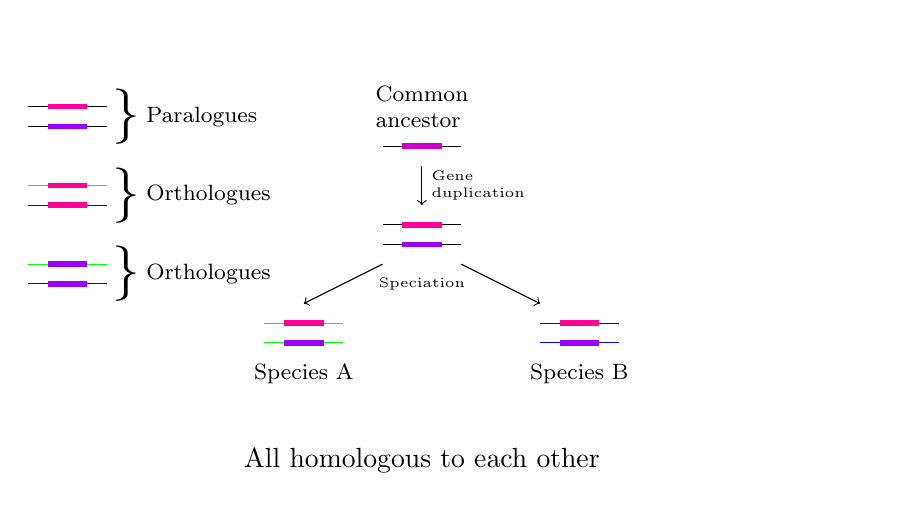
\begin{tikzpicture}[scale=0.5]
      \draw [help lines, opacity=0] (0,0) grid (22,12);
%     \foreach \x in {1,2,...,19} \node [font=\small] at (\x,0) {\x};
%     \foreach \y in {1,2,...,12} \node [font=\small] at (20,\y) {\y};
      \visible<2->{
        \node [align=left, font=\footnotesize] at (10,10) {Common\\ancestor};
        \draw [-] (9,9) -- (11,9);
        \draw [-,line width=2, purple2] (9.5,9) -- (10.5,9);
      }
      \visible<3->{
        \draw [->] (10,8.5) -- (10,7.5) node [midway, right, align=left, font=\tiny] 
        {Gene\\duplication};
        \genePair{10}{7}
      }
      \visible<4->{
        \draw [->] (9,6) -- (7,5);
        \draw [->] (11,6) -- (13,5);
        \node [font=\tiny] at (10,5.5) {Speciation};
        \genePair[green]{7}{4.5}
        \genePair[blue]{14}{4.5}
        \node [font=\footnotesize] at (7,3.2) {Species A};
        \node [font=\footnotesize] at (14,3.2) {Species B};
      }
      \visible<5->{
        \genePair{1}{10};
        \node [scale=2] at (2.5,9.75) {\}};
        \node [right, font=\footnotesize] at (2.75, 9.75) {Paralogues};
      }
      \visible<6->{
        \draw [-,green] (0,8) -- (2,8);
        \draw [-,blue] (0,7.5) -- (2,7.5);
        \draw [-,purple1, line width=2] (0.5,8) -- (1.5,8);
        \draw [-,purple1, line width=2] (0.5,7.5) -- (1.5,7.5);
        \node [scale=2] at (2.5,7.75) {\}};
        \node [right, font=\footnotesize] at (2.75,7.75) { Orthologues };
        
        \draw [-,green] (0,6) -- (2,6);
        \draw [-,blue] (0,5.5) -- (2,5.5);
        \draw [-,purple3, line width=2] (0.5,6) -- (1.5,6);
        \draw [-,purple3, line width=2] (0.5,5.5) -- (1.5,5.5);
        \node [scale=2] at (2.5,5.75) {\}};
        \node [right, font=\footnotesize] at (2.75,5.75) { Orthologues };
      }
      \visible<7->{
        \node at (10,1) {All homologous to each other};
      }
    \end{tikzpicture}
  \end{figure}
\end{frame}

\begin{frame}{Multiple Alignment. More whys}
  Addresses many biological questions and technical issues:
  \begin{itemize}
  \item diagnostic patterns for protein families
  \item detect or demonstrate homology between sequences
  \item help predict secondary and tertiary structures
  \item to suggest oligonucleotide primers for PCR
  \item essential prelude to molecular evolutionary analysis
  \item ...
  \end{itemize}
  \blfootnote{Shamelessly copied from Thompson et al., NAR 1994 22(22): 4673-4680\\
    \url{http://www.ncbi.nlm.nih.gov/pmc/articles/PMC308517/}
  }
\end{frame}

\begin{frame}{How to align many sequences?}
  In theory, possible to use dynamic programming algorithms (eg. Needleman-Wunsch,
  Smith Waterman) to find optimal alignments.

  But the complexity of these scale by $l^n$ (where $l$ is the length of the sequences,
  and $n$ is the number of sequences). Too complex both in terms of memory
  requirements and 
  processing time for more than a few sequences. (But examples exist).

  \textcolor{navy}{\emph{Heuristic}} methods are used instead. These do not guarantee an
  optimal result, but provide sufficient speed.

  Many methods exist: we will look in detail at one of these.
\end{frame}

\begin{frame}{ClustalW}
  \begin{figure}[ht]
    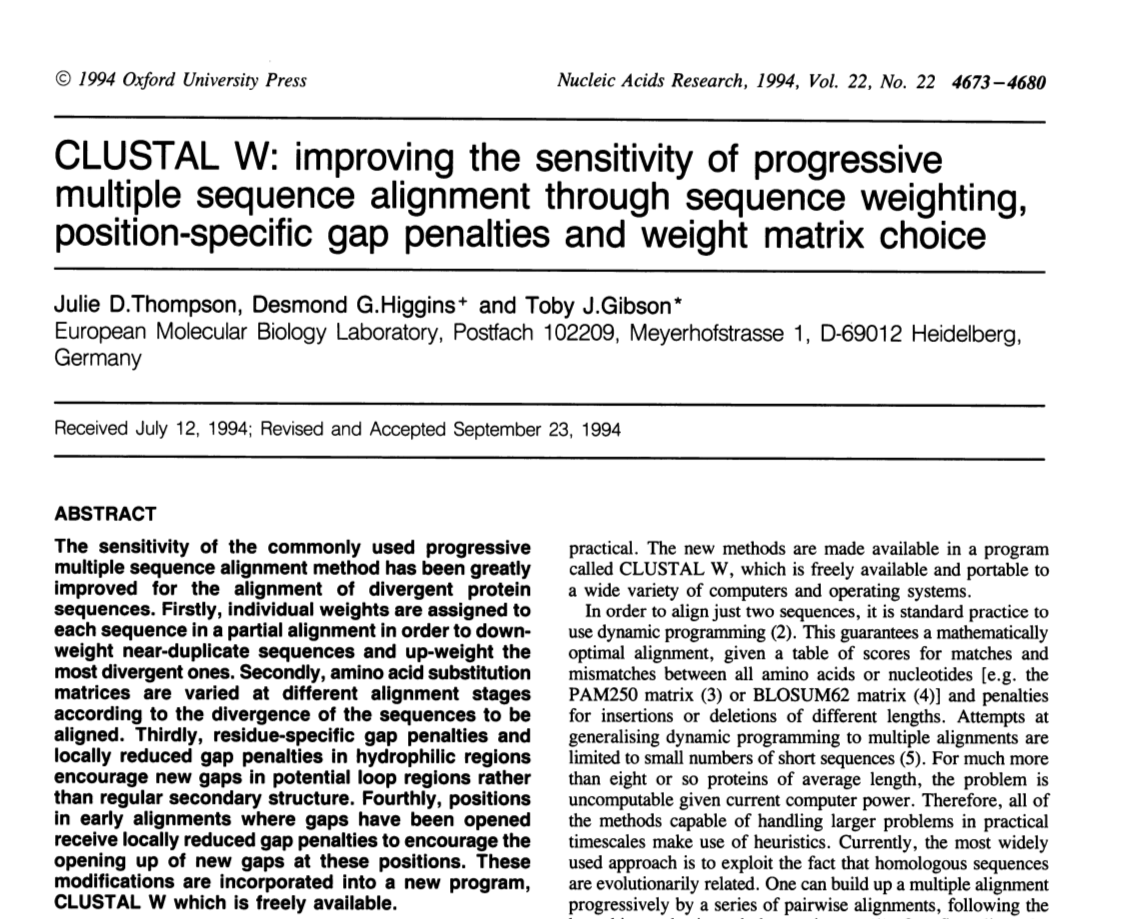
\includegraphics[width=0.9\textwidth]{images/clustalw_title}
  \end{figure}
\end{frame}

\begin{frame}{Why ClustalW}
  \begin{itemize}
    \item One of the most widely used methods
    \item Easy to understand
    \item Includes phylogenetic analysis
    \item Paper describes the derivation and reasoning for the heuristics used
      nicely (eg. this can be a 
      problem, so we tweaked this part of the method to give nicer results).
    \item The method extends naturally from pairwise alignment.
  \end{itemize}

\end{frame}

\begin{frame}{The clustal method}
  For a collection of sequences:
  \begin{enumerate}
  \item Align all pairs of sequences and calculate a distance matrix (table).
  \item Use the distance matrix to calculate a guide tree.
  \item Align the sequences progressively according to the branch order
    of the guide tree.
  \end{enumerate}
\end{frame}

\begin{frame}{Pairwise alignment}
  \begin{itemize}
  \item Global alignment of all pairs using a modification of Needleman-Wunsch,
    or a faster k-tuple based heuristic method.
  \item Scores are calculated as: number of identities / number of residues compared
    (gap positions are excluded).
  \item Distances are are simply (1 - score)
  \end{itemize}

  This gives an n by n distance matrix which is then used to make a guiding tree.
\end{frame}

\begin{frame}{The guide tree}
  Tree created from the distances to represent the similarities between the
  sequences and to suggest an order for the progressive alignment. 

  Earlier versions used UPGMA. Newer version uses Neighbor joining algorithm.

\end{frame}

\begin{frame}{What is a tree}
  \begin{itemize}
  \item A way to represent a set of relationships (commonly distances or dis-similarities).
  \item Often obtained by hierarchical clustering methods from distances matrices (see below).
  \item Can also be obtained by maxium parsimony or maximum expectation methods.
  \item Originally developed to represent evolutionary relationships (i.e. phylogenetic trees).
  \item Now also used to summarise N-dimensional data sets in general (covered later in the course).
  \end{itemize}
\end{frame}

\begin{frame}{UPGMA: the simplest tree}
  Unweighted Pair Group Method with Arithmetic Mean
  \begin{figure}[ht]
    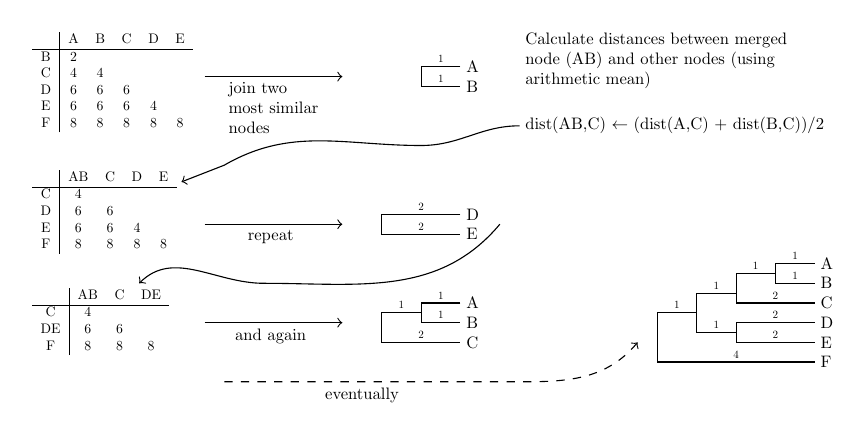
\begin{tikzpicture}[scale=0.5]
%     \draw [help lines, opacity=1] (0,0) grid (22,12);
%     \foreach \x in {1,2,...,19} \node [font=\small] at (\x,0) {\x};
%     \foreach \y in {1,2,...,12} \node [font=\small] at (20,\y) {\y};
     
     \node [below right, scale=0.5] at (0,12) {
       \begin{tabular}{ c| ccccc }
         & A & B & C & D & E \\
         \hline
         B & 2 &&&& \\
         C & 4 & 4 &&& \\
         D & 6 & 6 & 6 && \\
         E & 6 & 6 & 6 & 4 & \\
         F & 8 & 8 & 8 & 8 & 8 
       \end{tabular}
     };
     \visible<2->{
       \draw [->] (4.5,10.75) -- (8,10.75) node [midway, below, align=left, scale=0.6]
       { join two\\most similar\\nodes };
       \draw [-] (11,11) node [right, scale=0.6] {A} -- (10,11) node [midway, above, scale=0.4] {1}
       -- (10,10.5) -- (11,10.5) node [midway, above, scale=0.4] {1};
       \node [right, scale=0.6] at (11,10.5) {B};
     }
     \visible<3->{
       \node [below right, align=left, scale=0.6, text width=6cm] at (12.5,12) {
         Calculate distances between merged node (AB) and other nodes (using arithmetic mean)};
       \node [right, scale=0.6] (eq1) at (12.5,9.5) 
       {dist(AB,C) $\leftarrow$ (dist(A,C) + dist(B,C))/2};
     };         
     
     \visible<4->{
       \node [below right, scale=0.5] (mat2) at (0,8.5) {
         \begin{tabular}{ c| cccc }
           & AB & C & D & E \\
           \hline
           C & 4 &&& \\
           D & 6 & 6 && \\
           E & 6 & 6 & 4 & \\
           F & 8 & 8 & 8 & 8 
         \end{tabular} };
       \draw [->] (eq1) to [out=180,in=0] (10,9) 
       to [out=180,in=30] (5,8.5) -- (mat2); 
     }
     \visible<5->{
       \draw [->] (4.5,7) -- (8,7) node [midway, below, align=left, scale=0.6]
       { repeat };
       \draw [-] (11,7.25) node [right, scale=0.6] {D} -- (9,7.25) node [midway, above, scale=0.4] {2}
       -- (9,6.75) -- (11,6.75) node [midway, above, scale=0.4] {2};
       \node [right, scale=0.6] at (11,6.75) {E};
     }
     \visible<6->{
       \node [below right, scale=0.5] (mat3) at (0,5.5) {
         \begin{tabular}{ c| ccc }
           &  AB & C & DE \\
           \hline
           C  & 4 && \\
           DE & 6 & 6 & \\
           F  & 8 & 8 & 8 
         \end{tabular} };
       \draw [->] (12,7) to [out=230,in=0] (6,5.5) to [out=180,in=45] (mat3);
     }
     \visible<7->{
       \draw [->] (4.5,4.5) -- (8,4.5) node [midway, below, align=left, scale=0.6]
       { and again };
       \draw [-] (11,5) node [right, scale=0.6] {A} -- (10,5) node [midway, above, scale=0.4] {1}
       -- (10,4.5) -- (11,4.5) node [midway, above, scale=0.4] {1};
       \node [right, scale=0.6] at (11,4.5) {B};
       \draw [-] (10,4.75) -- (9,4.75) node [midway, above, scale=0.4] {1}
       -- (9,4) -- (11,4) node [midway, above, scale=0.4] {2};
       \node [right, scale=0.6] at (11,4) {C};
     }
     \visible<8->{
       \draw [->, dashed] (5,3) -- (12,3) node [pos=0.5, below, scale=0.6] {eventually}
       to [out=0,in=230] (15.5,4);
       \draw [-] (20,6) node [right, scale=0.6] {A} -- (19,6) node [midway, above, scale=0.4] {1}
       -- (19,5.5) -- (20,5.5) node [midway, above, scale=0.4] {1};
       \node [right, scale=0.6] at (20,5.5) {B};
       \draw [-] (19,5.75) -- (18,5.75) node [midway, above, scale=0.4] {1}
       -- (18,5) -- (20,5) node [midway, above, scale=0.4] {2};
       \node [right, scale=0.6] at (20,5) {C};
       \draw [-] (18,5.25) -- (17,5.25) node [midway, above, scale=0.4] {1}
       -- (17,4.25) -- (18,4.25) node [midway, above, scale=0.4] {1}
       -- (18,4.5) -- (20,4.5) node [midway, above, scale=0.4] {2};
       \draw (20,4) -- (18,4) node [midway, above, scale=0.4] {2} -- (18,4.25);
       \draw (17,4.75) -- (16,4.75) node [midway, above, scale=0.4] {1}
       -- (16,3.5) -- (20,3.5) node [midway, above, scale=0.4] {4};
       \node [right, scale=0.6] at (20,4.5) {D};
       \node [right, scale=0.6] at (20,4) {E};
       \node [right, scale=0.6] at (20,3.5) {F};
     }
   \end{tikzpicture}
 \end{figure}
  \blfootnote{Scheme adapted from:\\
    \url{http://www.icp.ucl.ac.be/~opperd/private/upgma.html}
  }
\end{frame}

\begin{frame}{Neighbor joining algorithm}
  \begin{itemize}
  \item Underlying algorithm method similar to UPGMA (i.e. progressively merge
    neighboring nodes until a single tree is obtained).
  \item Modified distance matrix used to find nearest nodes to join.
  \item Distances of pair members to joins are influenced by distances to external nodes.
  \item Does not assume equal rate of evolution\\ $\Rightarrow$ neighbours have
    differing distances to their joining nodes.
  \item Better than UPGMA (?)
  \end{itemize}
\blfootnote{Saitou and Nei, Mol Biol Evol 1987, Jul;4(4);406-25}  
\end{frame}

\begin{frame}{Neighbor joining (1)}
  Nodes to be joined (i.e. neighbors) are chosen from a Q matrix:
  $$
  Q_{i,j} = (n-2)d_{i,j} - \sum_{k=1}^n{d_{i,k}} - \sum_{k=1}^n{d_{j,k}}
  $$
  Where $d_{i,j}$ is the distance between the $i^{th}$ and $j^{th}$ nodes, $n$ is
  the total number of nodes.

  This will preferentially select outlier pairs to join (i.e. pairs of nodes
  which are distant from the larger set).
\end{frame}

\begin{frame}{Neighbor joining (2)}
  The pair with the lowest pair $Q$ value are joined through a new node. If we refer to the
  neighbors as $f$ and $g$, and the new (joining) node as $u$, then we calculate the distance
  between new node and $f$ and $g$ by:
  \begin{equation}
    \begin{aligned}
      & \delta_{f,u} = \frac{1}{2}d_{f,g} +
      \frac{1}{2(n-2)}\Bigg[\sum_{k=1}^n{d_{f,k}} - \sum_{k=1}^n{d_{g,k}}
        \Bigg] \\
      & \delta_{g,u} = d_{f,g} - \delta_{f,u}
    \end{aligned}
  \end{equation}
  $\delta_{f,u}$ and $\delta_{g,u}$ the distances between $f$ and $g$ and the
  joining node $u$ are adjusted such that they are proportional to their
  respective distances to the remaining nodes.
\end{frame}

\begin{frame}{Neighbor joining (3)}
  The distances of the remaining nodes to the joining node $u$ are set as:
  $$
  \delta_{u,k} = \frac{1}{2}[d_{f,k} + d_{g,k} - d_{f,g}]
  $$
  where $u$ is the joining node, $k$ is each of the remaining nodes; $f$ and
  $g$ are the nodes joined as before.

  This assures that the total distance within the tree is consistent.

  \blfootnote{These equations taken from the Wikipedia page:\\
    \url{https://en.wikipedia.org/wiki/Neighbor_joining}\\
    They differ slightly in their form, but not substance from the original publication.}
\end{frame}

\begin{frame}{Neighbor joining: putting it together}
  \begin{enumerate}
  \item Determine the Q matrix based on the current distance matrix.
  \item Find the pair of nodes with the smallest Q value.
  \item Create a new node that connects this pair.
  \item Determine the distances of all the nodes to this new joining node.
  \item Replace the neighbour pair with the new node and update the distance
    matrix.
  \item Repeat from (1) until the tree is fully connected.
  \end{enumerate}
  
\end{frame}

\begin{frame}{Progressive alignment}
  \begin{figure}[ht]
    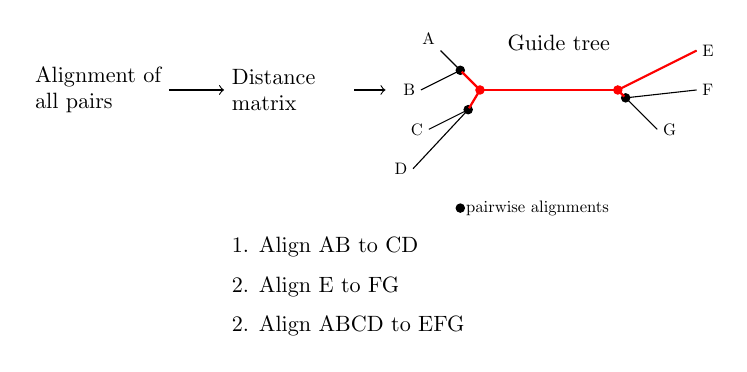
\begin{tikzpicture}[scale=0.5]
%      \draw [help lines, opacity=1] (0,0) grid (22,12);
%      \foreach \x in {1,2,...,19} \node [font=\small] at (\x,0) {\x};
%      \foreach \y in {1,2,...,12} \node [font=\small] at (20,\y) {\y};
      \node [right, align=left, scale=0.8] (al1) at (0,10) {Alignment of\\all
        pairs};
      \draw [->] (al1) -- (5,10) node (dm1)
            [right, align=left, scale=0.8] {Distance\\matrix};
      \draw [-] (10.5,11) node [above left, scale=0.6] {A} -- (11,10.5) node
            [inner sep=0, outer sep=0] (j1) {} -- (10,10) node [left,
              scale=0.6] {B};
      \draw [->] (8.3,10) -- (9.1,10);
      \node [scale=0.8] at (13.5,11.2) {Guide tree};
      \draw [-] (10.2,9) node [left, scale=0.6] {C} -- (11.2,9.5) node [inner
        sep=0, outer sep=0] (j2) {} -- (9.8,8) node [left, scale=0.6] {D};
      \draw [-] (j1) -- (11.5,10) node (j3) [inner sep=0, outer sep=0] {} -- (j2) ;
      \draw [-] (j3) -- (15,10) node (j4) [inner sep=0, outer sep=0] {} --
      (17,11) node (E) [right, scale=0.6] {E};
      \draw [-] (j4) -- (15.2,9.8) node (j5) [inner sep=0, outer sep=0] {} --
      (16,9) node (G) [right, scale=0.6] {G} ;
      \draw [-] (j5) -- (17,10) node [right, scale=0.6] {F};
      \visible<2->{
        \filldraw (j1) circle (3pt);
        \filldraw (j2) circle (3pt);
        %%\filldraw (j3) circle (3pt);
        %%\filldraw (j4) circle (3pt);
        \filldraw (j5) circle (3pt);
        \node [right, scale=0.6] at (11,7) {pairwise alignments};
        \filldraw (11,7) circle (3pt);
      }
      \visible<3->{
        \draw [thick, red] (j1) -- (j3) -- (j2);
        \filldraw [red] (j3) circle (3pt);
        \node [right, scale=0.8] at (5,6) {1. Align AB to CD};
      }
      \visible<4->{
        \draw [thick, red] (17,11) -- (j4) -- (j5);
        \filldraw [red] (j4) circle (3pt);
        \node [right, scale=0.8] at (5,5) {2. Align E to FG};
      }
      \visible<5->{
        \draw [thick, red] (j3) -- (j4);
        %\filldraw [red] (j4) circle (3pt);
        \node [right, scale=0.8] at (5,4) {2. Align ABCD to EFG};
      }
      
    \end{tikzpicture}
  \end{figure}
  \visible<6->{
    How to align two alignments?
  }

\end{frame}

\begin{frame}[fragile]{Aligning alignments}
  Modify the scoring function to use several sequences.
  
  Match score is set to the mean of all independent pairs:
  \begin{figure}[ht]
    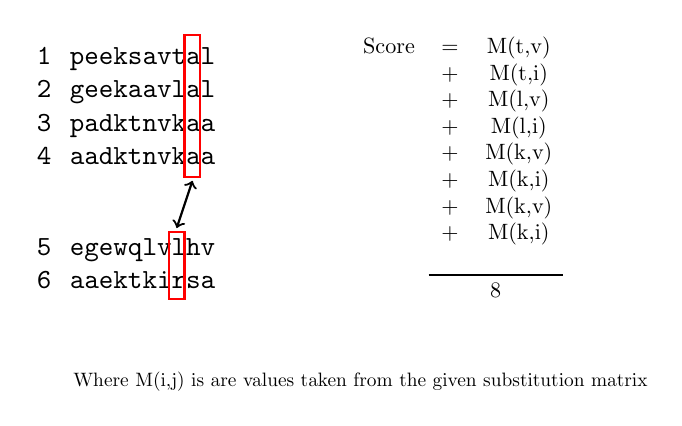
\begin{tikzpicture}[scale=0.5]
%      \draw [help lines, opacity=0.3] (0,0) grid (22,12);
%      \foreach \x in {1,2,...,19} \node [font=\small] at (\x,0) {\x};
%      \foreach \y in {1,2,...,12} \node [font=\small] at (20,\y) {\y};
      \node [right, text width=13em] at (1,8) {
        \verb|1  peeksavtal|
        \verb|2  geekaavlal|
        \verb|3  padktnvkaa|
        \verb|4  aadktnvkaa|
      };
      \node [right, text width=13em] at (1,4) {
        \verb|5  egewqlvlhv|
        \verb|6  aaektkirsa|
      };
      \visible<2->{
        \draw [thick, red] (5,6.2) rectangle (5.4,9.8);
        \draw [thick, red] (4.6,3.1) rectangle (5,4.8);
        \draw [<->, thick] (5.2,6.1) -- (4.8,4.9);
      }
      \visible<3->{
        \node [below right, scale=0.8] at (9,10) {
          \begin{tabular}{ccc}
            Score & = & M(t,v) \\
            & + & M(t,i) \\
            & + & M(l,v) \\
            & + & M(l,i) \\
            & + & M(k,v) \\
            & + & M(k,i) \\
            & + & M(k,v) \\
            & + & M(k,i)
          \end{tabular}
        };
        \draw [-,thick] (11.2,3.7) -- (14.6,3.7) node [midway, below, scale=0.8] {8};
        \node [right, scale=0.7] at (2,1) {Where M(i,j) is are values taken
          from the given substitution matrix};
      }
    \end{tikzpicture}
  \end{figure}
    
\end{frame}

\begin{frame}{Refinements}
  This describes the basic method and should be sufficient to provide
  reasonable multiple sequence alignments.\\
  For difficult sets of sequences (eg. with little similarity) a number
  of refinements have been incorporated into the method.
  \small
  \begin{itemize}
  \item Weighting of sequences to correct for unequal sampling across
    evolutionary distances in the data set (greater weight to outlier sequences)
  \item Dynamic variation of gap penalties (to mimic known tendencies in
    proteins)
    \begin{itemize}
    \item Increase gap opening penalty within 8 amino acid of a gap opening
    \item Decrease gap opening penalty in hydrophilic stretches (associated
      with loops)
    \item Decreased gap opening penalties at positions of gaps in early
      alignments.
    \end{itemize}
  \item Dynamic use of weight matrices: starting with weight matrices suitable
    for closely related sequences and moving to divergent weight matrices.
  \end{itemize}
\end{frame}

\begin{frame}{Problems?}
  \begin{itemize}
    \item All alignments are global alignments and it may be necessary to
      trim sequences to give reasonable alignments.
    \item The guide tree is based on a matrix of distances of seperately aligned
      trees and may not be reliable. This may lead to mistakes early in the
      merging process that cannot be corrected later.
  \end{itemize}
  
\end{frame}

\begin{frame}{works ok!}
  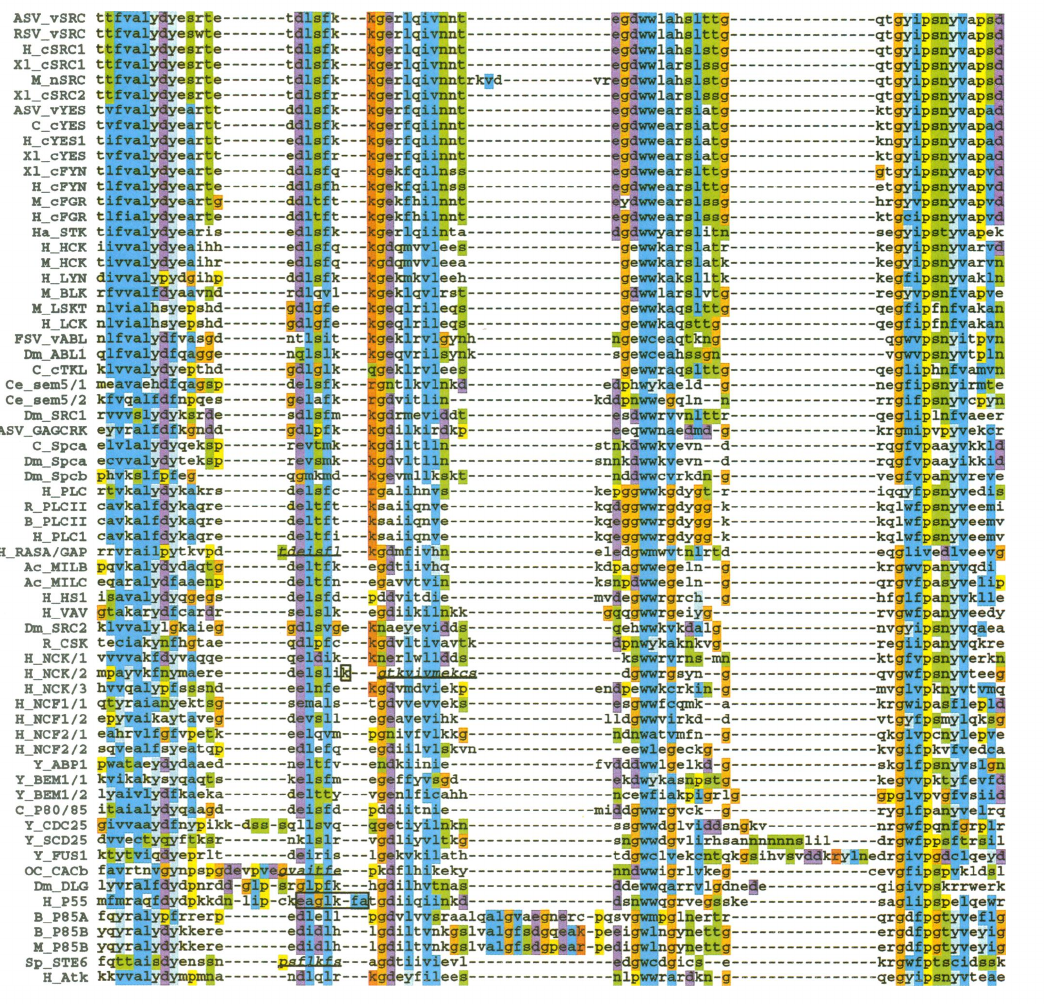
\includegraphics[width=0.8\textwidth]{images/clustal_alignment}
\end{frame}

\begin{frame}{Other methods}
  \footnotesize
  \begin{itemize}
  \item DCA. Semi-exhaustive, divide and conquer algorithm. Breaks sequences
    into segments based on local similarity. Segments are aligned by dynamic
    programming and then joined.\\
    \href{http://bibiserv.techfak.uni-bielefeld.de/dca?id=dca\_view\_webservice}
    {bibiserv.techfak.uni-bielefeld.de/dca?id=dca\_view\_webservice}
  \item Poa (Partial order alignments). Uses a graph representation of the
    multiple alignment that can be aligned by dynamic programming.\\
    \href{http://bioinformatics.oxfordjournals.org/content/18/3/452.short}
    {bioinformatics.oxfordjournals.org/content/18/3/452.short}
  \item Dialign (and Dialign2, Dialign-TX). Compares segments of sequences rather 
    than individual residues without using gap penalties. Good for comparing
    sequences with only local similarity.\\
   \href{http://mobyle.pasteur.fr/cgi-bin/portal.py?\#forms::dialign}
   {mobyle.pasteur.fr/cgi-bin/portal.py?\#forms::dialign}
  \item Can also be achieved by probabilistic methods (eg. Hidden Markov Models),
    though these are normally used to model (describe) sequences rather than to
    perform the actual alignment. But see hmmbuild:\\
    \href{http://hmmer.janelia.org/}{hmmer.janelia.org/}
  \end{itemize}

  Many more available. Method usually determined by the sheep algorithm
  (i.e. use what others in the field are using).
  
\end{frame}

\end{document}

